We also created a tool that gives the option to the animators to display the results of the BVH files into a panel in the form of an mp4. In particular, we convert the information that we get from the motion data into an mp4, and then we display it to the user.  This procedure is quite simple. We read from the BVH file the Skeleton information, as well as the motion data. We use the matplotlib library that allows us to create a 3D space, and we import into that space all the keypoints for each frame. Therefore, we have completed our algorithm. The animators can convert any human video that meets our requirements into a BVH file. Then they can clear the motion data, with the tool that we are offering, and afterward render the animation into an avatar in order to import it to a Game Engine like Unity.  In the figure below someone can see the input video that someone wants to extract the motion compared to the visualization that we created, the visualization that Blender offers, and finally the motion inside a Game Engine when it is rendered into a humanoid avatar.

\pagebreak

\begin{figure}[htp]
    \centering
    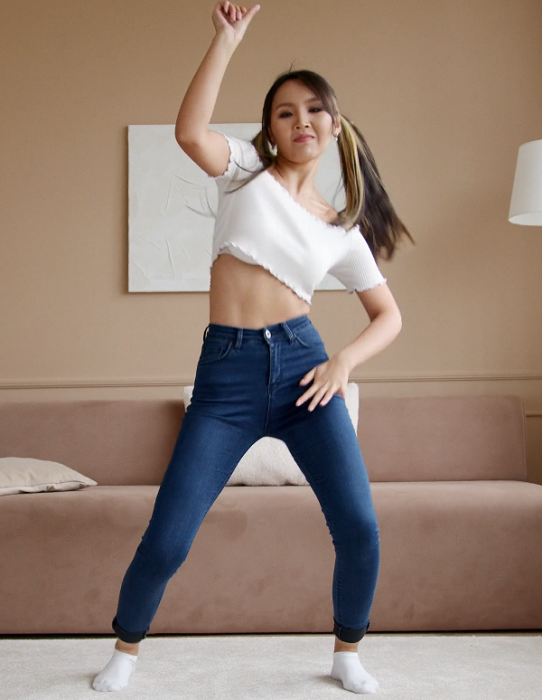
\includegraphics[width=0.35\textwidth]{figures/Implementation/videoplayer1.png}%
    \qquad
    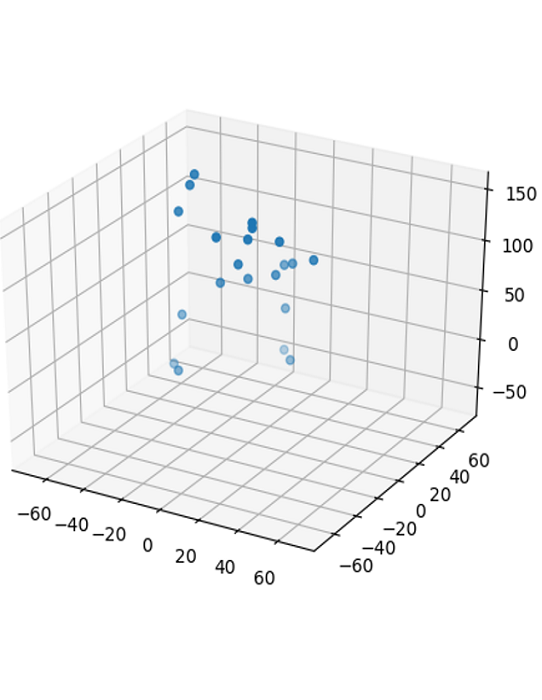
\includegraphics[width=0.35\textwidth]{figures/Implementation/videoplayer2.png}%
    \qquad
    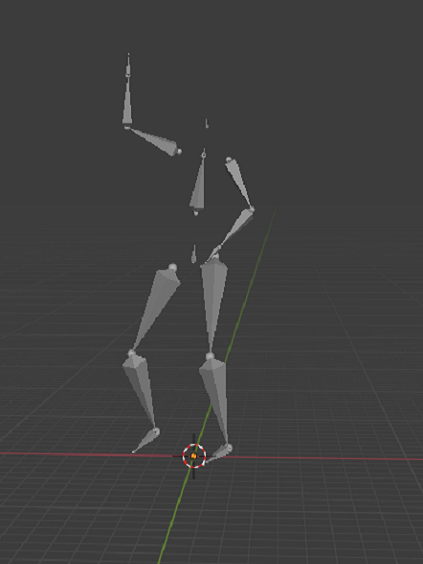
\includegraphics[width=0.35\textwidth]{figures/Implementation/videoplayer3.png}%
    \qquad
    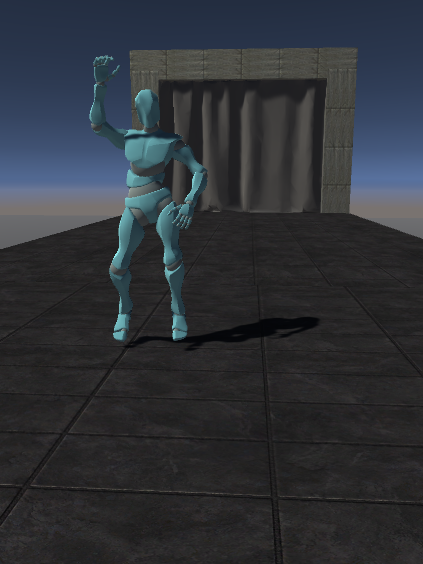
\includegraphics[width=0.35\textwidth]{figures/Implementation/videoplayer4.png}%
    \captionsetup{labelformat=empty}
    \caption{We display a frame from the input video, and the estimated BVH file, in both our video player and Blender. Finally, we display the BVH file when we clean it, convert it into an FBX file, and import it to Unity.}%
\end{figure}

\subsubsection*{Rendering an Avatar to the BVH file}

At this point, we completed the second phase of this Thesis. The final phase is to create a more friendly environment for the user that will use these algorithms and tools. The last image of the above figure is the desired output that we want, the FBX file. This file is the BVH file that we created when we render it into an avatar. More specifically, the FBX file, in our case, is a motioned BVH Skeleton with humanoid skin. Someone can find these skins on some online websites, like mixamo, that's where we got the skin in that image, or he can create his own avatar in studios like Blender. There are some other online applications where someone can find an avatar like Polycom, it is an application that allows you to create high-quality 3D models from photos with any mobile phone. For a Humanoid 3D model it may need many photos but someone can create an avatar that looks like himself, and if we combine it with our thesis, someone can convert his real-life motion into a computerized humanoid avatar that has his form and motion.